\documentclass[10pt]{beamer}

\usepackage{fontspec}
\setmainfont{Roboto Mono}[]
\setsansfont{Roboto Mono}[]
\setmonofont{Roboto Mono}[]

\usepackage{graphicx}
\graphicspath{ {../img/} }

\usepackage[absolute,overlay]{textpos} % [showboxes]

\beamertemplatenavigationsymbolsempty

\usepackage{listings}
\lstset{
  language=ML,
  keywordstyle=\color{blue},
  backgroundcolor=\color{lightgray}
}

\title{Связь между процессами}

\begin{document}

\begin{frame}
  \frametitle{Fault Tolerance}
  Устойчивость к ошибкам основана на:
  \begin{itemize}
    \item связях между процессами: link и monitor,
    \item системных сообщениях (сигналах),
    \item разделении на системные и рабочие процессы.
  \end{itemize}
\end{frame}

\begin{frame}[fragile]
  \frametitle{link и spawn\_link}
  \begin{lstlisting}
  Process.link/1
  Process.unlink/1
  Kernel.spawn_link/3
  \end{lstlisting}
\end{frame}

\begin{frame}[fragile]
  \frametitle{Системные процессы}
  \begin{lstlisting}
  Process.flag(:trap_exit, true)
  \end{lstlisting}
\end{frame}

\begin{frame}[fragile]
  \frametitle{exit}
  \begin{lstlisting}
  Process.exit(pid, reason)
  \end{lstlisting}
\end{frame}

\begin{frame}
  \frametitle{exit reason}
  \begin{itemize}
    \item normal,
    \item kill,
    \item любая другая
  \end{itemize}
\end{frame}

\begin{frame}
  \frametitle{Варианты событий при завершении процесса}
  \center
  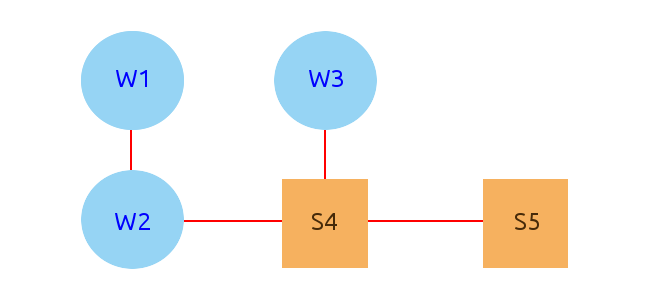
\includegraphics[scale=0.2]{link_exit_1}
\end{frame}

\begin{frame}
  \frametitle{normal exit}
  \center
  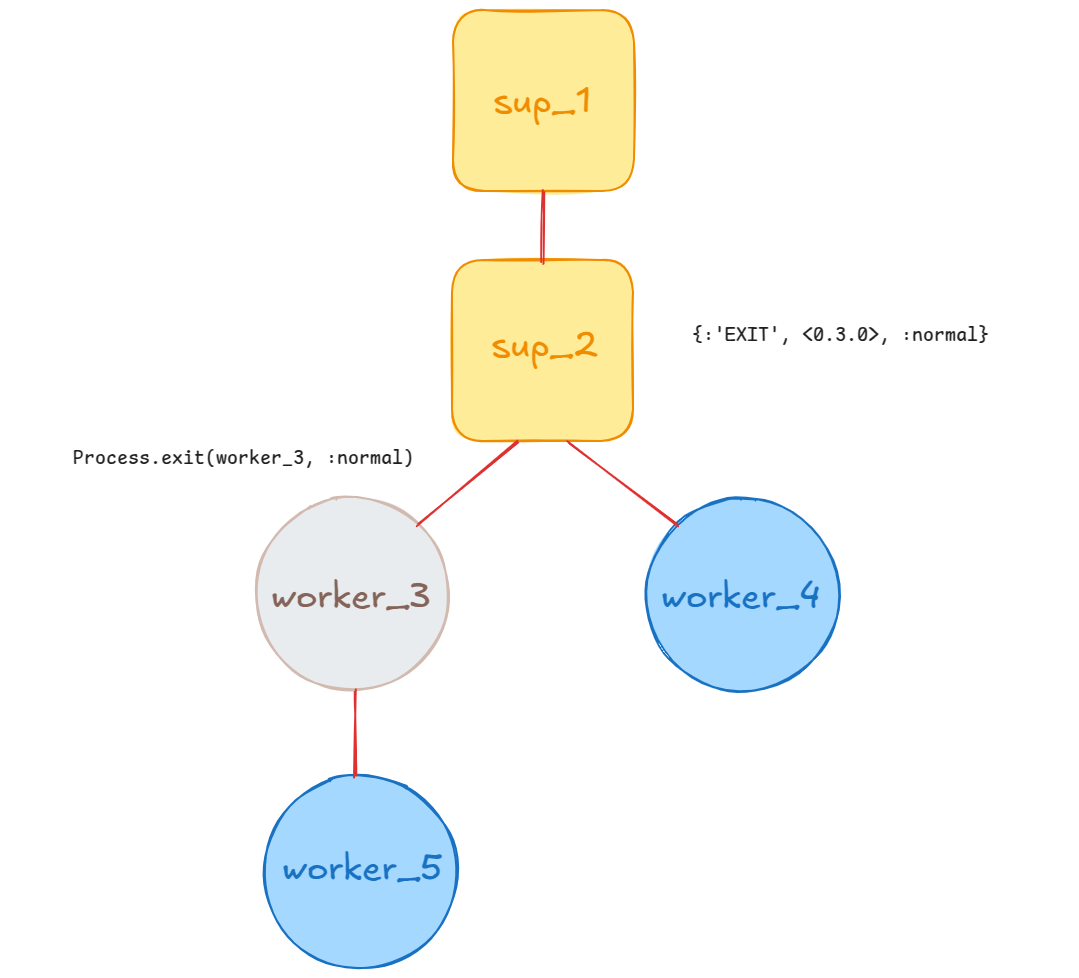
\includegraphics[scale=0.2]{link_exit_2}
\end{frame}

\begin{frame}
  \frametitle{not normal exit}
  \center
  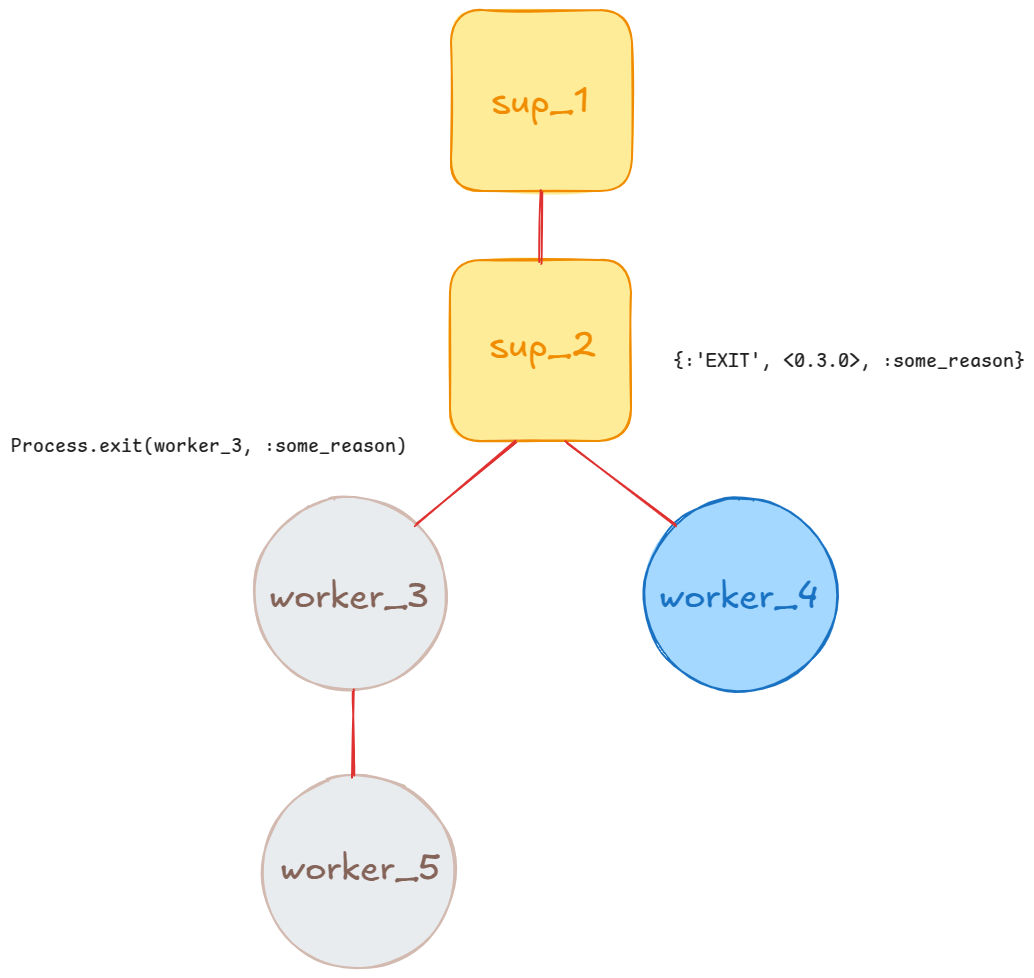
\includegraphics[scale=0.2]{link_exit_3}
\end{frame}

\begin{frame}
  \frametitle{exit with kill}
  \center
  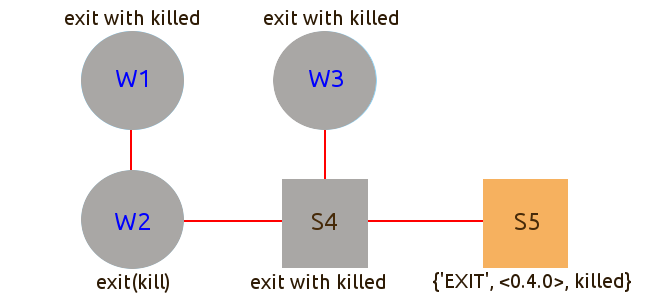
\includegraphics[scale=0.2]{link_exit_4}
\end{frame}

\end{document}
